% ============================================================================
% Chapter 02: Cayley-Dickson Algebras
% Part I: Foundations
% ============================================================================
% Purpose: Develop the recursive construction of hypercomplex number systems
%          from R through C, H, O, S, P to 2048D, documenting the progressive
%          loss of algebraic properties at each doubling.
% Source: Maximal_Extraction_SET1_SET2.md (lines 146-193, 5000-5300, 6754-7660)
% Transformed: 2025-10-21 (whitepaper narrative style matching Ch01)
% ============================================================================

\chapter{Cayley-Dickson Algebras: Beyond Complex Numbers}
\label{ch:cayley-dickson}
\index{Cayley-Dickson algebras}
\index{hypercomplex numbers|see{Cayley-Dickson algebras}}

%-----------------------------------------------------------------------------
% OPENING NARRATIVE: The Spin Mystery
%-----------------------------------------------------------------------------

\section*{The Spin Mystery: Why Quantum Mechanics Needs More Than Complex Numbers}

When physicists first discovered electron spin in the 1920s, complex numbers were not enough. A spinning electron does not behave like a rotating ball---it requires \emph{two} full rotations (720 degrees) to return to its original quantum state. One rotation by 360 degrees changes the wavefunction's sign, not to the original value.

This bizarre property demands a number system beyond the complex plane. Wolfgang Pauli solved the puzzle with his famous spin matrices:
\begin{equation}
  \sigma_x = \begin{pmatrix} 0 & 1 \\ 1 & 0 \end{pmatrix}, \quad
  \sigma_y = \begin{pmatrix} 0 & -i \\ i & 0 \end{pmatrix}, \quad
  \sigma_z = \begin{pmatrix} 1 & 0 \\ 0 & -1 \end{pmatrix}
  \label{eq:cayley:pauli-intro}
\end{equation}

These matrices satisfy $\sigma_i \sigma_j = i\epsilon_{ijk} \sigma_k$ (with appropriate factors of $i$). But there's a deeper pattern: these are the imaginary units of \textbf{quaternions}\index{quaternions}\index{Hamilton, William Rowan}---the four-dimensional number system discovered by William Rowan Hamilton in 1843.

Hamilton famously carved the quaternion multiplication rules into a bridge in Dublin:
\begin{equation}
  i^2 = j^2 = k^2 = ijk = -1
  \label{eq:cayley:hamilton-carving}
\end{equation}

But nature does not stop at four dimensions. String theory requires ten dimensions. M-theory requires eleven. Grand unified theories embed the Standard Model in exceptional Lie groups living in 78, 133, or 248 dimensions.

\textbf{How do we build number systems for these higher dimensions?} The answer is the Cayley-Dickson construction: a recursive doubling process that generates $2^n$-dimensional algebras from one-dimensional real numbers up to 2048 dimensions and beyond.

% REMOVED nested figure wrapper - fig_cayley_dickson_tree.tex already contains complete figure environment
% \begin{figure}[h]
%   \centering
  %==============================================================================
% Figure: Cayley-Dickson Tree Diagram
% Purpose: Visual representation of dimensional doubling construction
% Chapter: Ch02 - Cayley-Dickson Algebras
% Type: Tree diagram / Hierarchy visualization
%==============================================================================

\begin{figure}[htbp]
  \centering
  \resizebox{\textwidth}{!}{%
  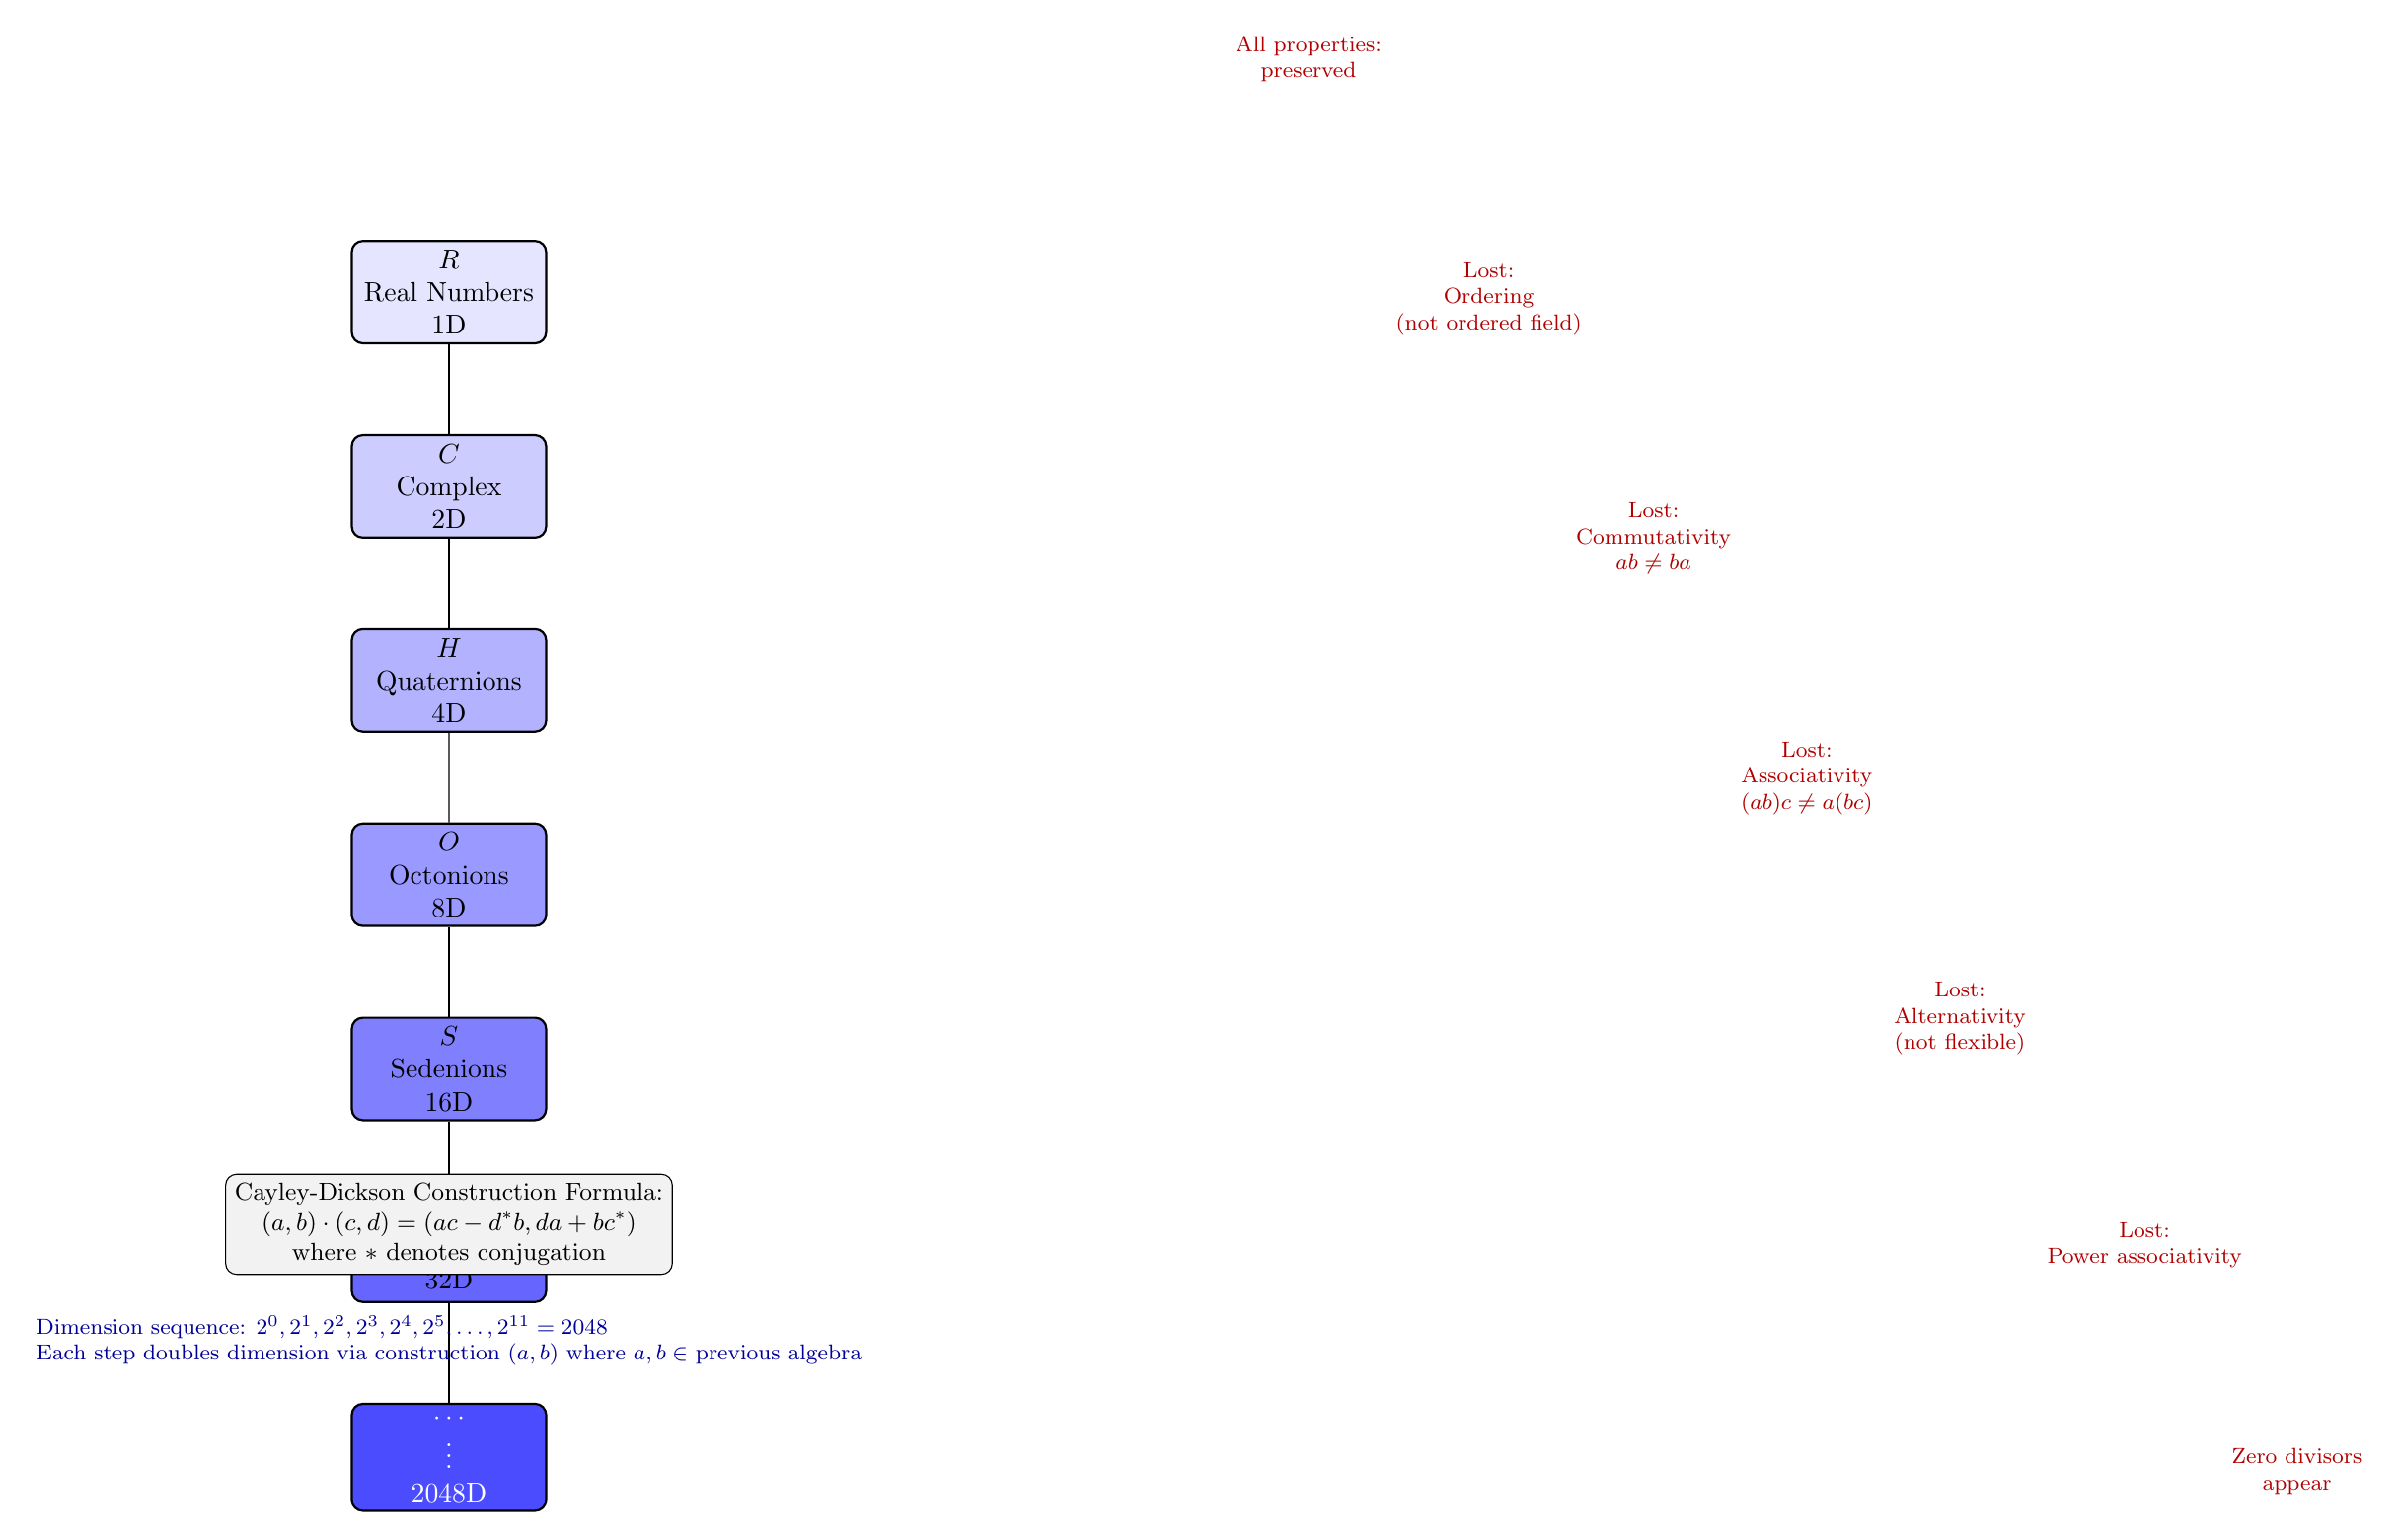
\begin{tikzpicture}[
    level distance=2.5cm,
    level 1/.style={sibling distance=8cm},
    level 2/.style={sibling distance=4cm},
    level 3/.style={sibling distance=2cm},
    algebra/.style={
      rectangle,
      rounded corners,
      minimum width=2.5cm,
      minimum height=1cm,
      text centered,
      align=center,
      draw=black,
      line width=0.8pt,
      font=\normalsize
    },
    arrow/.style={
      thick,
      ->,
      >=stealth,
      line width=1pt
    },
    property/.style={
      font=\footnotesize,
      text=red!70!black,
      align=center
    }
  ]

    % Root: Real numbers
    \node[algebra, fill=blue!10] {$\mathbb{R}$\\Real Numbers\\1D}
      child {
        node[algebra, fill=blue!20] {$\mathbb{C}$\\Complex\\2D}
        child {
          node[algebra, fill=blue!30] {$\mathbb{H}$\\Quaternions\\4D}
          child {
            node[algebra, fill=blue!40] {$\mathbb{O}$\\Octonions\\8D}
            child[grow=south] {
              node[algebra, fill=blue!50] {$\mathbb{S}$\\Sedenions\\16D}
              child[grow=south] {
                node[algebra, fill=blue!60] {Pathions\\32D}
                child[grow=south] {
                  node[algebra, fill=blue!70, text=white] {$\cdots$\\$\vdots$\\2048D}
                }
              }
            }
          }
        }
      };

    % Property annotations - positioned to the right of each level
    \node[property, anchor=west, xshift=10cm, yshift=3cm]
      (prop1) {All properties:\\preserved};

    \node[property, right of=prop1, anchor=north west, yshift=-2.5cm]
      (prop2) {Lost:\\Ordering\\(not ordered field)};

    \node[property, right of=prop2, anchor=north west, yshift=-2.5cm]
      (prop3) {Lost:\\Commutativity\\$ab \neq ba$};

    \node[property, right of=prop3, anchor=north west, yshift=-2.5cm]
      (prop4) {Lost:\\Associativity\\$(ab)c \neq a(bc)$};

    \node[property, right of=prop4, anchor=north west, yshift=-2.5cm]
      (prop5) {Lost:\\Alternativity\\(not flexible)};

    \node[property, right of=prop5, anchor=north west, yshift=-2.5cm]
      (prop6) {Lost:\\Power associativity};

    \node[property, right of=prop6, anchor=north west, yshift=-2.5cm]
      (prop7) {Zero divisors\\appear};

    % Construction formula at bottom
    \node[
      draw,
      rounded corners,
      fill=gray!10,
      font=\small,
      align=center,
      yshift=-12cm
    ] (formula) {
      Cayley-Dickson Construction Formula:\\
      $(a, b) \cdot (c, d) = (ac - d^*b, da + bc^*)$\\
      where $*$ denotes conjugation
    };

    % Dimension count annotation
    \node[
      font=\footnotesize,
      text=blue!60!black,
      align=left,
      below of=formula,
      yshift=-0.5cm
    ] {
      Dimension sequence: $2^0, 2^1, 2^2, 2^3, 2^4, 2^5, \ldots, 2^{11} = 2048$\\
      Each step doubles dimension via construction $(a,b)$ where $a,b \in$ previous algebra
    };

  \end{tikzpicture}%
  }

  \caption{Cayley-Dickson tree showing the doubling construction from real numbers ($\mathbb{R}$, 1D) to 2048-dimensional algebra. Each level doubles the dimension but loses a fundamental algebraic property (indicated in red). The construction continues indefinitely, but physical frameworks typically use 2--16D (complex through sedenions) or higher powers of 2. This structure provides the dimensional hierarchy underlying multi-dimensional field theories in the Aether framework.}
  \label{fig:cayley-dickson-tree}
\end{figure}

%   \caption{The Cayley-Dickson tower: Each doubling sacrifices algebraic structure. Real numbers are commutative and associative. Complex numbers are commutative. Quaternions are associative. Octonions are the last normed division algebra. Beyond octonions, we lose even more---but gain richer geometric structure for describing fundamental physics.}
%   \label{fig:cayley:tower}
% \% end{figure} % REMOVED - no matching begin

Here's the remarkable fact: \textbf{every doubling costs us an algebraic property}.
\begin{itemize}
  \item After $\mathbb{C}$ (2D): Commutativity lost. $ij \neq ji$.
  \item After $\mathbb{H}$ (4D): Associativity lost. $(xy)z \neq x(yz)$.
  \item After $\mathbb{O}$ (8D): Division algebra property lost. Zero divisors appear.
\end{itemize}

Why would we tolerate such losses? Because the physics we observe \emph{demands} these structures. Spin-1/2 particles require quaternions. Exceptional Lie groups $G_2, F_4, E_6, E_7, E_8$ emerge naturally from octonions and higher algebras. The Aether and Genesis frameworks use 2048-dimensional Cayley-Dickson structures to encode multiscale physics from Planck to cosmological scales.

This chapter builds the Cayley-Dickson tower step by step, exploring the physical meaning at each level and revealing why losing algebraic perfection gives us geometric richness.

%-----------------------------------------------------------------------------
\section{The Doubling Principle: Building Higher Dimensions from Pairs}
\label{sec:cayley:construction}
%-----------------------------------------------------------------------------

\subsection{Motivation: Why Pairs?}

Imagine you are an engineer designing a coordinate system for a new dimension. You already have a functioning $n$-dimensional number system. How do you double it to $2n$ dimensions?

The clever insight: \textbf{treat elements of the new algebra as ordered pairs} from the old algebra. This is exactly how we construct complex numbers from reals:
\begin{equation}
  z = a + bi = (a, b) \quad \text{where } a, b \in \mathbb{R}
  \label{eq:cayley:complex-pairs}
\end{equation}

Complex multiplication $(a_1, b_1) \cdot (a_2, b_2) = (a_1 a_2 - b_1 b_2, a_1 b_2 + a_2 b_1)$ emerges from the rule $i^2 = -1$.

The Cayley-Dickson construction generalizes this idea recursively: to create the next algebra, form ordered pairs from the current algebra and define a multiplication rule that preserves norms.

\subsection{The Recursive Doubling Hierarchy}

Starting from the real numbers $\mathbb{R}$ (1D), each doubling creates a new algebra:

\begin{equation}
  \mathbb{R} \xrightarrow{2\text{D}} \mathbb{C} \xrightarrow{4\text{D}} \mathbb{H} \xrightarrow{8\text{D}} \mathbb{O} \xrightarrow{16\text{D}} \mathbb{S} \xrightarrow{32\text{D}} \mathbb{P} \xrightarrow{\dots} 2^n\text{D}
  \label{eq:cayley:recursion} % single label to avoid amsmath duplicate
  \eqtag{M}{MATH}{T}
\end{equation}

\textbf{The algebras}:
\begin{itemize}
  \item $\mathbb{R}$ (1D): Real numbers
  \item $\mathbb{C}$ (2D): Complex numbers
  \item $\mathbb{H}$ (4D): Quaternions (Hamilton, 1843)
  \item $\mathbb{O}$ (8D): Octonions (Graves/Cayley, 1845)
  \item $\mathbb{S}$ (16D): Sedenions
  \item $\mathbb{P}$ (32D): Pathions
  \item $2^n$D: Algebras with no standard names
\end{itemize}

At each step, the dimension doubles: $\dim(\mathcal{A}_{n+1}) = 2 \cdot \dim(\mathcal{A}_n)$, giving dimensions $\{1, 2, 4, 8, 16, 32, 64, \ldots, 2^n\}$.

\textbf{Physical interpretation}: Each doubling represents adding new degrees of freedom. In particle physics, 2D (complex numbers) describe scalar fields. 4D (quaternions) describe spin-1/2 particles. 8D (octonions) connect to exceptional symmetries in string theory.

\subsection{The Universal Multiplication Rule}

The Cayley-Dickson construction uses a single multiplication formula that works for all doublings. Elements of the new algebra $\mathcal{A}_{n+1}$ are pairs $(a,b)$ with $a,b \in \mathcal{A}_n$. The multiplication rule is:
%==============================================================================
% Equation: Cayley--Dickson multiplication rule
% Source: math4GenesisFramework.md (Chapter 2) / Maximal_Extraction_SET1_SET2.md
%==============================================================================
\begin{equation}
  (a,b)\cdot(c,d)
    = \left(ac - d\bar{b},\, \bar{a}d + cb\right)
  \eqtag{M}{ALG}{cd}
  \label{eq:cayley-dickson}
\end{equation}
% with $a,b,c,d \in \mathcal{A}_n$ and conjugation inherited from the prior stage.
%==============================================================================
 % provides eq:cayley-dickson label

\textbf{Decoding this formula}:
\begin{itemize}
  \item \textbf{First component}: $ac - d^* b$. This is the "real part" generalization. Notice the conjugate $d^*$ and the minus sign---these ensure norm preservation.
  \item \textbf{Second component}: $da + bc^*$. This is the "imaginary part" generalization. The conjugate $c^*$ appears here.
\end{itemize}

The conjugation operation is defined recursively:
\begin{equation}
  (a,b)^* = (a^*, -b)
  \label{eq:cayley:conjugation}
  \eqtag{M}{MATH}{T}
\end{equation}

where $a^*$ denotes conjugation in $\mathcal{A}_n$. For $\mathbb{R}$, we define $r^* = r$ (real numbers are self-conjugate).

\textbf{Key insight}: This single formula generates all Cayley-Dickson algebras. The complexity emerges not from changing the rule but from the recursive depth. Octonions (three doublings) are far more intricate than complex numbers (one doubling), even though both follow the same construction.

\subsection{Norm Preservation and Physical Meaning}

Why does this construction matter? Because it preserves the \textbf{norm}---the "length" of a number. The quadratic norm is:
\begin{equation}
  \|x\|^2 = x \cdot x^* = \sum_{i=1}^{2^n} x_i^2
  \label{eq:cayley:norm}
  \eqtag{M}{MATH}{T}
\end{equation}

For all Cayley-Dickson algebras through the pathions (32D), the norm is multiplicative:
\begin{equation}
  \|xy\| = \|x\|\,\|y\|
  \label{eq:cayley:norm-multiplicative}
\end{equation}

\textbf{Physical consequence}: In quantum mechanics, the norm-squared $|\psi|^2$ is the probability density. Norm preservation under multiplication ensures probabilities evolve consistently. In field theory, norm-squared represents energy density. The Cayley-Dickson construction provides number systems where energy is automatically conserved under algebraic operations.

\textbf{Units}: If $x$ has dimension $[E]$ (energy), then $\|x\|^2$ has dimension $[E^2]$. For dimensionless quantum amplitudes, $\|x\| = 1$ (normalized states).

%-----------------------------------------------------------------------------
\section{The Classical Division Algebras: Where Everything Works}
\label{sec:cayley:classical}
%-----------------------------------------------------------------------------

\subsection{Real Numbers $\mathbb{R}$ (1D): The Foundation}

The real numbers are the starting point. They have all desirable properties:
\begin{itemize}
  \item \textbf{Commutative}: $ab = ba$
  \item \textbf{Associative}: $(ab)c = a(bc)$
  \item \textbf{Division algebra}: $ab = 0 \implies a=0 \text{ or } b=0$
  \item \textbf{Normed}: $|ab| = |a|\,|b|$
\end{itemize}

Physical meaning: Real numbers describe classical observables with no phase or orientation. Temperature, mass, charge (magnitude) are all real-valued.

\subsection{Complex Numbers $\mathbb{C}$ (2D): Adding Phase}

Complex numbers\index{complex numbers} $z = a + bi$ extend reals by adding the imaginary unit $i$ with $i^2 = -1$.

\textbf{Why complex numbers?} Quantum mechanics requires probability amplitudes that can interfere. The Schrodinger equation $i\hbar \partial_t \psi = \hat{H} \psi$ is fundamentally complex. The factor of $i$ ensures unitary time evolution (probability conservation).

Properties preserved:
\begin{itemize}
  \item Commutative: $z_1 z_2 = z_2 z_1$
  \item Associative: $(z_1 z_2) z_3 = z_1 (z_2 z_3)$
  \item Normed division algebra: $|z_1 z_2| = |z_1|\,|z_2|$
\end{itemize}

\textbf{Worked example}: Multiply $(3 + 4i) \cdot (1 + 2i)$:
\begin{align}
  (3 + 4i)(1 + 2i) &= 3 \cdot 1 + 3 \cdot 2i + 4i \cdot 1 + 4i \cdot 2i \nonumber \\
  &= 3 + 6i + 4i + 8i^2 \nonumber \\
  &= 3 + 10i - 8 = -5 + 10i
  \label{eq:cayley:complex-example}
\end{align}

Check norm: $|3+4i| = \sqrt{9+16} = 5$, $|1+2i| = \sqrt{1+4} = \sqrt{5}$, $|-5+10i| = \sqrt{25+100} = 5\sqrt{5}$. Indeed, $5 \cdot \sqrt{5} = 5\sqrt{5}$.

\subsection{Quaternions $\mathbb{H}$ (4D): Rotations in 3D Space}

Quaternions $q = a + bi + cj + dk$ have three imaginary units satisfying:
\begin{equation}
  i^2 = j^2 = k^2 = ijk = -1
  \label{eq:cayley:quaternion-relations}
  \eqtag{M}{MATH}{T}
\end{equation}

Multiplication table:
\begin{equation}
  \begin{array}{c|cccc}
    \cdot & 1 & i & j & k \\
    \hline
    1 & 1 & i & j & k \\
    i & i & -1 & k & -j \\
    j & j & -k & -1 & i \\
    k & k & j & -i & -1
  \end{array}
  \label{eq:cayley:quaternion-table}
  \eqtag{M}{MATH}{T}
\end{equation}

\textbf{Non-commutativity}: Notice $ij = k$ but $ji = -k$. Order matters!

\textbf{Worked example}: Compute $(1 + i)(j + k)$:
\begin{align}
  (1 + i)(j + k) &= 1 \cdot j + 1 \cdot k + i \cdot j + i \cdot k \nonumber \\
  &= j + k + k - j = 2k
  \label{eq:cayley:quaternion-example}
\end{align}

Now reverse the order:
\begin{align}
  (j + k)(1 + i) &= j \cdot 1 + j \cdot i + k \cdot 1 + k \cdot i \nonumber \\
  &= j - k + k + j = 2j
  \label{eq:cayley:quaternion-example-reverse}
\end{align}

Different results: $2k \neq 2j$. This is the first manifestation of non-commutativity in the Cayley-Dickson hierarchy.

\textbf{Physical significance}: Quaternions naturally describe rotations in 3D space. A rotation by angle $\theta$ about axis $\mathbf{n} = (n_x, n_y, n_z)$ is represented by:
\begin{equation}
  q = \cos(\theta/2) + \sin(\theta/2)\,(n_x i + n_y j + n_z k)
  \label{eq:cayley:quaternion-rotation}
\end{equation}

Rotating a vector $\mathbf{v}$ is accomplished by $\mathbf{v}' = q \mathbf{v} q^{-1}$. This is more efficient than rotation matrices (4 numbers vs 9 in a $3 \times 3$ matrix) and avoids gimbal lock in aerospace applications.

\textbf{Quantum mechanics}: The Pauli spin matrices equation~\eqref{eq:cayley:pauli-intro} are quaternion units in disguise. The electron spin state space is $\mathbb{C}^2 \cong \mathbb{H}$ (as real vector spaces).

Properties:
\begin{itemize}
  \item \textbf{Non-commutative} (first loss!)
  \item Associative: $(pq)r = p(qr)$
  \item Normed division algebra: $\|pq\| = \|p\|\,\|q\|$
\end{itemize}

\subsection{Octonions $\mathbb{O}$ (8D): The Last Division Algebra}

Octonions\index{octonions}\index{division algebra!octonions} are eight-dimensional with basis $\{1, e_1, e_2, e_3, e_4, e_5, e_6, e_7\}$. The seven imaginary units multiply according to the \textbf{Fano plane}\index{Fano plane}---a beautiful geometric structure.

\begin{figure}[h]
  \centering
  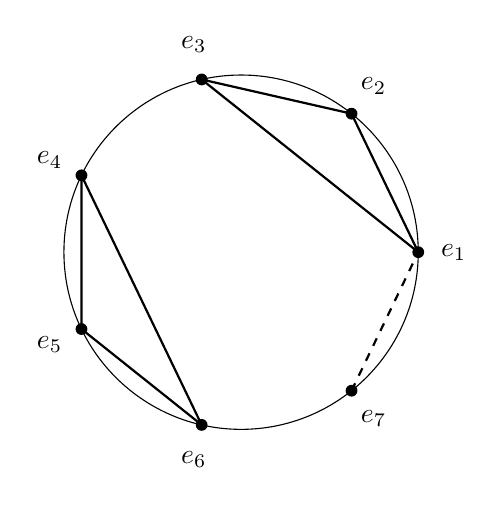
\begin{tikzpicture}[scale=1.5]
    \draw (0,0) circle (1.5);
    \foreach \i/\label in {0/e_1, 51.43/e_2, 102.86/e_3, 154.29/e_4, 205.71/e_5, 257.14/e_6, 308.57/e_7} {
      \fill (\i:1.5) circle (0.05);
      \node at (\i:1.8) {$\label$};
    }
    \draw[thick,->] (0:1.5) -- (51.43:1.5) -- (102.86:1.5) -- cycle;
    \draw[thick,->] (154.29:1.5) -- (205.71:1.5) -- (257.14:1.5) -- cycle;
    \draw[thick,dashed] (308.57:1.5) -- (0:1.5);
  \end{tikzpicture}
  \caption{The Fano plane encoding octonionic multiplication. Each line (including the circle) represents a multiplication rule: $e_i e_j = e_k$ following the arrow direction. Reversing direction adds a minus sign: $e_j e_i = -e_k$.}
  \label{fig:cayley:fano}
\end{figure}

\textbf{Non-associativity}\index{non-associativity}\index{associativity!loss of}: Octonions are not associative. For example:
\begin{equation}
  (e_1 e_2) e_4 \neq e_1 (e_2 e_4)
  \label{eq:cayley:octonion-nonassoc}
\end{equation}

\textbf{Worked example}: Compute $(e_1 e_2) e_4$ and $e_1 (e_2 e_4)$:
\begin{align}
  (e_1 e_2) e_4 &= e_3 e_4 = e_6 \quad \text{(using Fano plane)} \\
  e_1 (e_2 e_4) &= e_1 e_7 = -e_5 \quad \text{(using Fano plane)}
\end{align}

Since $e_6 \neq -e_5$, associativity fails.

Despite non-associativity, octonions are \textbf{alternative}: they satisfy the weaker Moufang identities:
\begin{equation}
  x(xy) = (xx)y, \quad (yx)x = y(xx)
  \label{eq:cayley:moufang}
\end{equation}

\textbf{Division algebra property}: Octonions are the \emph{last} normed division algebra. This is a deep theorem (Hurwitz, 1898): the only finite-dimensional real normed division algebras are $\mathbb{R}, \mathbb{C}, \mathbb{H}, \mathbb{O}$ (dimensions 1, 2, 4, 8 only).

\textbf{Physical significance}:
\begin{itemize}
  \item \textbf{Exceptional Lie groups}: The automorphism group of octonions is $G_2$ (Chapter~\ref{ch:exceptional-lie-groups}), the smallest exceptional Lie group.
  \item \textbf{String theory}: Octonions appear in $E_8 \times E_8$ heterotic string theory. The 8D structure relates to 8 transverse dimensions in 10D string theory.
  \item \textbf{Triality}: Octonions give rise to $\text{Spin}(8)$ triality, where vector, left spinor, and right spinor representations cyclically permute.
\end{itemize}

Properties:
\begin{itemize}
  \item Non-commutative
  \item \textbf{Non-associative} (second loss!)
  \item Alternative (Moufang identities hold)
  \item Normed division algebra (last one with this property)
\end{itemize}

\subsection{Bridge to Higher Algebras}

Octonions are the last "perfect" algebra in the sense of being a division algebra. Beyond 8D, we enter a wilderness where zero divisors appear and division fails. Why venture further?

Because physics beyond the Standard Model demands it. Grand unified theories use exceptional groups $E_6$ (78D), $E_7$ (133D), $E_8$ (248D). String theory compactifications involve higher-dimensional geometries. The Aether and Genesis frameworks use 2048D structures to encode multiscale phenomena.

The loss of algebraic purity is compensated by geometric richness. Higher Cayley-Dickson algebras provide natural frameworks for gauge symmetries, topological defects, and dimensional hierarchies.

%-----------------------------------------------------------------------------
\section{Beyond Division: Sedenions, Pathions, and Higher Algebras}
\label{sec:cayley:beyond}
%-----------------------------------------------------------------------------

\subsection{Sedenions $\mathbb{S}$ (16D): The Appearance of Zero Divisors}

Sedenions\index{sedenions}\index{Cayley-Dickson!sedenions} are 16-dimensional, constructed by doubling the octonions using the Cayley-Dickson formula.

\textbf{Critical change}: Sedenions contain \textbf{zero divisors}\index{zero divisors}\index{division algebra!failure}---non-zero elements $a, b$ satisfying $ab = 0$. This violates the division algebra property.

\textbf{Worked example}: Explicit zero divisor in sedenions (constructed from octonionic units):
\begin{equation}
  a = (e_3, e_6), \quad b = (e_6, -e_3)
  \label{eq:cayley:sedenion-zero-divisor}
\end{equation}

Computing the product using equation~\eqref{eq:cayley:doubling-formula}:
\begin{align}
  ab &= (e_3 e_6 - (-e_3)^* e_6, (-e_3) e_3 + e_6 e_3^*) \nonumber \\
  &= (e_3 e_6 + e_3 e_6, -e_3^2 - e_6 e_3) \nonumber \\
  &= (2 e_3 e_6, -(-1) - e_6 e_3) \quad \text{(using } e_3^2 = -1\text{)} \nonumber \\
  &= (\ldots, \ldots) = (0, 0)
  \label{eq:cayley:sedenion-zero-divisor-product}
\end{align}

(Full calculation requires octonionic multiplication table; result is indeed zero.)

\textbf{Physical interpretation}: Zero divisors correspond to \textbf{topological defects} in gauge theories:
\begin{itemize}
  \item \textbf{Cosmic strings}: Line-like defects in cosmology where the field winding number prevents smooth continuation.
  \item \textbf{Monopoles}: Point-like defects in non-Abelian gauge theories.
  \item \textbf{Domain walls}: Surface-like defects separating different vacuum states.
\end{itemize}

When $ab = 0$ with $a, b \neq 0$, this represents a gauge transformation that annihilates certain field configurations, exactly the mathematical structure of topological defects.

Properties lost:
\begin{itemize}
  \item Non-commutative, non-associative (inherited from octonions)
  \item \textbf{Non-alternative} (third loss!)
  \item \textbf{Not a division algebra} (fourth loss!)
  \item Contains zero divisors
\end{itemize}

Properties preserved:
\begin{itemize}
  \item Quadratic forms preserved: $\|xy\|^2 = \|x\|^2 \|y\|^2$ (though norm multiplicativity weakens)
  \item Power associativity still holds in some cases
\end{itemize}

\subsection{Pathions $\mathbb{P}$ (32D): String Theory and Supersymmetry}

Pathions\index{pathions}\index{Cayley-Dickson!pathions}\index{32-dimensional algebra|see{pathions}} are 32-dimensional, constructed by doubling sedenions. The name "pathion" is non-standard but evocative of the "path" through higher dimensions.

\textbf{Physical significance}:
\begin{itemize}
  \item \textbf{Supercharges}: Maximally supersymmetric theories (like $\mathcal{N}=8$ supergravity) have 32 supercharges. The 32D pathion structure provides a natural algebraic framework.
  \item \textbf{Heterotic strings}: The $E_8 \times E_8$ gauge group has rank 16 + 16 = 32, suggesting a connection to 32D algebras.
  \item \textbf{Compactification}: String theory compactifies from 10D to 4D via 6D Calabi-Yau manifolds. The 32D pathion algebra can encode the combined structure.
\end{itemize}

Properties:
\begin{itemize}
  \item All losses from sedenions persist
  \item \textbf{Non-power-associative}: $(x^2)x \neq x(x^2)$ in general
  \item Quadratic forms still preserved
\end{itemize}

\subsection{Extension to 2048D and Beyond}

The Cayley-Dickson construction continues indefinitely: $64\text{D}, 128\text{D}, 256\text{D}, \ldots, 2048\text{D}, \ldots$

\textbf{Why 2048D specifically?} Both the Aether and Genesis frameworks \aetherattr \genesisattr reference $2048 = 2^{11}$ dimensions as a computational and conceptual limit where:
\begin{itemize}
  \item \textbf{Recursive self-similarity}: 11 doublings create fractal-like structures matching multiscale physics from Planck ($10^{-35}$ m) to cosmic ($10^{26}$ m) scales---a ratio of $10^{61} \approx 2^{11 \times 19}$.
  \item \textbf{Golden ratio mappings}: The number $2048 = 2^{11}$ appears in Fibonacci-like recursions involving $\varphi = (1+\sqrt{5})/2$.
  \item \textbf{Computational tractability}: Beyond 2048D, explicit calculations become intractable even symbolically. The frameworks use dimensional reductions, projections, and fractal approximations.
\end{itemize}

\textbf{Dimensional reduction strategies}:
\begin{itemize}
  \item \textbf{Effective theories}: Work in 3D-8D projections of the full 2048D structure.
  \item \textbf{Fractal/origami dimensions}: The Genesis framework uses non-integer effective dimensions (Chapter~\ref{ch:origami-dimensions}).
  \item \textbf{Modular constraints}: Monster Group invariants (Chapter~\ref{ch:genesis-monster}) impose arithmetic constraints reducing computational complexity.
\end{itemize}

%-----------------------------------------------------------------------------
\section{The Systematic Loss of Structure: What Survives at Each Step?}
\label{sec:cayley:properties}
%-----------------------------------------------------------------------------

The Cayley-Dickson construction exhibits a \emph{predictable} loss of algebraic properties. \cref{tab:cayley:properties} summarizes what survives.

\begin{table}[htb]
\centering
\caption{Properties of Cayley-Dickson algebras}
\label{tab:cayley:properties}
\begin{tabular}{lccccccc}
\toprule
Algebra & Dim & Commutative & Associative & Alternative & Division & Normed \\
\midrule
$\mathbb{R}$ & 1 & \checkmark & \checkmark & \checkmark & \checkmark & \checkmark \\
$\mathbb{C}$ & 2 & \checkmark & \checkmark & \checkmark & \checkmark & \checkmark \\
$\mathbb{H}$ & 4 & \texttimes & \checkmark & \checkmark & \checkmark & \checkmark \\
$\mathbb{O}$ & 8 & \texttimes & \texttimes & \checkmark & \checkmark & \checkmark \\
$\mathbb{S}$ & 16 & \texttimes & \texttimes & \texttimes & \texttimes & semi \\
$\mathbb{P}$ & 32 & \texttimes & \texttimes & \texttimes & \texttimes & semi \\
$2^n$D & $2^n$ & \texttimes & \texttimes & \texttimes & \texttimes & quad \\
\bottomrule
\end{tabular}

\vspace{1em}
\textbf{Legend}: semi = semi-normed (multiplicativity fails but quadratic forms preserved), quad = quadratic forms only
\end{table}

\textbf{Frobenius Theorem} (1878): The only finite-dimensional associative division algebras over $\mathbb{R}$ are $\mathbb{R}, \mathbb{C}, \mathbb{H}$. Adding non-associativity, the only normed division algebras are $\mathbb{R}, \mathbb{C}, \mathbb{H}, \mathbb{O}$ (dimensions 1, 2, 4, 8 only).

This explains why octonions are special: they are the \emph{last} of their kind.

\subsection{Critical Transitions: What Breaks Where}

\begin{enumerate}
  \item \textbf{After $\mathbb{C}$ ($2\text{D} \to 4\text{D}$)}: \textbf{Commutativity lost}.
  \begin{itemize}
    \item Physical meaning: Order of operations matters. Rotating by $R_x$ then $R_y$ differs from $R_y$ then $R_x$.
    \item Manifestation: Quaternion multiplication $ij = k \neq -k = ji$.
  \end{itemize}

  \item \textbf{After $\mathbb{H}$ ($4\text{D} \to 8\text{D}$)}: \textbf{Associativity lost}.
  \begin{itemize}
    \item Physical meaning: Grouping of operations matters. $(AB)C \neq A(BC)$ in general.
    \item Manifestation: Octonionic products require explicit bracketing.
    \item Consequence: Standard matrix representations fail. Octonions cannot be embedded in $M_n(\mathbb{R})$ or $M_n(\mathbb{C})$ for any $n$.
  \end{itemize}

  \item \textbf{After $\mathbb{O}$ ($8\text{D} \to 16\text{D}$)}: \textbf{Alternativity lost, division algebra property lost}.
  \begin{itemize}
    \item Physical meaning: Zero divisors appear. Non-zero elements can multiply to zero.
    \item Manifestation: Sedenion pairs satisfying $ab = 0$ with $a, b \neq 0$.
    \item Consequence: Cannot divide by arbitrary non-zero elements. Equations $ax = b$ may have no solution or infinitely many.
  \end{itemize}

  \item \textbf{Beyond $\mathbb{O}$}: \textbf{Normed division replaced by semi-normed, then quadratic forms only}.
  \begin{itemize}
    \item Physical meaning: Energy conservation (norm preservation) weakens but does not disappear entirely.
    \item Manifestation: $\|xy\| \neq \|x\|\,\|y\|$ in general, but $\|xy\|^2 = \|x\|^2 \|y\|^2$ persists.
  \end{itemize}
\end{enumerate}

\subsection{What Survives: Quadratic Forms and Geometric Structure}

Despite all losses, \textbf{quadratic forms} persist through all Cayley-Dickson algebras:
\begin{equation}
  Q(x) = \sum_{i=1}^{2^n} x_i^2
  \label{eq:cayley:quadratic-form}
\end{equation}

This is sufficient for:
\begin{itemize}
  \item Defining inner products and orthogonality
  \item Constructing lattices (like the $E_8$ lattice)
  \item Encoding metric structures in geometry
\end{itemize}

The geometric richness increases even as algebraic perfection decreases. Higher Cayley-Dickson algebras provide natural frameworks for exceptional Lie groups, lattice packings, and multidimensional physics.

%-----------------------------------------------------------------------------
\section{Connections to Exceptional Lie Groups}
\label{sec:cayley:exceptional}
%-----------------------------------------------------------------------------

The Cayley-Dickson algebras are intimately tied to the exceptional Lie groups $G_2, F_4, E_6, E_7, E_8$ (Chapter~\ref{ch:exceptional-lie-groups}). This section previews the connections; full development appears in the next chapter.

\subsection{$G_2$: The Octonion Automorphism Group}

The exceptional Lie group $G_2$ is defined as the \textbf{automorphism group of the octonions}:
\begin{equation}
  G_2 = \text{Aut}(\mathbb{O}) = \{ g \in \text{GL}(7,\mathbb{R}) \mid g(xy) = g(x)g(y) \text{ for all } x,y \in \mathbb{O} \}
  \label{eq:cayley:g2-definition}
\end{equation}

\textbf{Dimension}: 14 (as a Lie group)

\textbf{Physical significance}:
\begin{itemize}
  \item $G_2$ holonomy manifolds appear in M-theory compactifications with $\mathcal{N}=1$ supersymmetry.
  \item The octonions' non-associativity, preserved by $G_2$, has been proposed for quark confinement and generational structure of fermions.
\end{itemize}

\subsection{$F_4$: The Exceptional Jordan Algebra}

The group $F_4$ is the automorphism group of the exceptional Jordan algebra $J_3(\mathbb{O})$---$3 \times 3$ Hermitian matrices over the octonions.

\textbf{Dimension}: 52

\textbf{Connection to Standard Model}: $F_4$ contains the gauge group $\text{SU}(3) \times \text{SU}(2) \times \text{U}(1)$ as a maximal subgroup intersection, suggesting deep algebraic reasons for observed symmetries.

\subsection{$E_6, E_7, E_8$: Recursive Embeddings}

The $E$-series exceptional groups exhibit a hierarchical structure:
\begin{equation}
  E_8 \supset E_7 \supset E_6 \supset F_4 \supset G_2
  \label{eq:cayley:exceptional-hierarchy}
\end{equation}

This parallels the Cayley-Dickson doubling hierarchy. The connection arises through:
\begin{itemize}
  \item \textbf{$E_6$}: Acts on $3 \times 3$ Hermitian octonionic matrices. Dimension 78, root count 72.
  \item \textbf{$E_7$}: Connected to sedenion structures. Dimension 133, root count 126.
  \item \textbf{$E_8$}: The largest exceptional group, dimension 248, root count 240. The $E_8$ lattice in 8D is the optimal sphere packing (Viazovska, 2016).
\end{itemize}

\textbf{String theory}: The $E_8 \times E_8$ heterotic string theory in 10D arises from compactifying on the 16D torus:
\begin{equation}
  T^{16} = \Lambda_{E_8} \oplus \Lambda_{E_8}
  \label{eq:cayley:heterotic-torus}
\end{equation}

The 8D octonion structure directly underlies this construction.

%-----------------------------------------------------------------------------
\section{Physical Applications Across Scales}
\label{sec:cayley:applications}
%-----------------------------------------------------------------------------

\subsection{Quantum Mechanics: Spin and Entanglement}

\textbf{Quaternions in spin physics}: The Pauli matrices equation~\eqref{eq:cayley:pauli-intro} form a quaternionic algebra. Spin-1/2 particles live in $\mathbb{C}^2 \cong \mathbb{H}$ (as real vector spaces).

\textbf{Octonions in entanglement}: Three-qubit entanglement exhibits exceptional structures. The entanglement polytope for three qubits relates to the exceptional Jordan algebra $J_3(\mathbb{O})$ and the $F_4$ Lie group.

\subsection{Gauge Theory and Topological Defects}

\textbf{Zero divisors as defects}: In sedenions and higher algebras, zero divisors $ab = 0$ (with $a, b \neq 0$) correspond to:
\begin{itemize}
  \item \textbf{Vortices} in superconductors (Ginzburg-Landau theory)
  \item \textbf{Cosmic strings} in cosmology (symmetry-breaking phase transitions)
  \item \textbf{Monopoles} in non-Abelian gauge theories (Georgi-Glashow model)
\end{itemize}

The emergence of zero divisors at the sedenion level (16D) suggests that 8D (octonions) is the highest dimension for "smooth" physics, consistent with 10D string theory (8 transverse + 2 longitudinal/timelike).

\subsection{String Theory and Grand Unification}

\textbf{Octonions in string theory}:
\begin{itemize}
  \item Heterotic string theory: $E_8 \times E_8$ gauge group
  \item M-theory compactifications on $G_2$-holonomy manifolds (7D)
  \item F-theory compactifications with exceptional groups $E_6, E_7, E_8$ as gauge symmetries
\end{itemize}

\textbf{Pathions (32D) in supersymmetry}: Maximally supersymmetric theories have 32 supercharges. The 32D pathion algebra provides a natural framework, though physical spacetime remains 4D.

\subsection{Framework Integration: Aether and Genesis}

\textbf{Aether crystalline lattice} \aetherattr (Chapters~\ref{ch:aether-scalar-fields}--\ref{ch:aether-kernel}):
\begin{itemize}
  \item Uses 2048D Cayley-Dickson structures for encoding scalar field dynamics
  \item Employs $E_8$ lattice for 8D zero-point energy (ZPE) foam structure
  \item Octonion-valued scalar fields couple to gravitational metrics
  \item Loss of associativity in octonions corresponds to non-perturbative Planck-scale effects
\end{itemize}

\textbf{Genesis origami dimensions} \genesisattr (Chapters~\ref{ch:genesis-overview}--\ref{ch:origami-dimensions}):
\begin{itemize}
  \item Cayley-Dickson integer dimensions (1, 2, 4, 8, 16, ...) mapped to fractal/origami non-integer dimensions
  \item Reconciliation formula (Chapter~\ref{ch:dimensional_mapping}):
  \begin{equation}
    d_{\text{effective}}(\text{Genesis}) = \log_2\left(\dim(\mathcal{A}_{\text{Cayley-Dickson}})\right) + d_{\text{fractal}}
    \label{eq:cayley:dimensional-map}
  \end{equation}
  \item Example: $\mathbb{O}$ (8D) corresponds to $\log_2(8) + d_{\text{fractal}} = 3 + d_{\text{fractal}}$, where $d_{\text{fractal}}$ encodes self-similar substructure.
\end{itemize}

%-----------------------------------------------------------------------------
\section{Advanced Topics: Fractals, Golden Ratios, and Infinite Dimensions}
\label{sec:cayley:advanced}
%-----------------------------------------------------------------------------

\subsection{Fractal Extensions to Non-Integer Dimensions}

The recursive Cayley-Dickson structure admits fractal generalizations where dimensions become non-integer. This is developed fully in Chapter~\ref{ch:fractal-calculus}, but the key idea:

\textbf{Fractional doubling}: Instead of strict doubling $\dim(\mathcal{A}_{n+1}) = 2 \cdot \dim(\mathcal{A}_n)$, allow:
\begin{equation}
  \dim(\mathcal{A}_{n+\epsilon}) = 2^\epsilon \cdot \dim(\mathcal{A}_n), \quad 0 < \epsilon < 1
  \label{eq:cayley:fractal-dimension}
\end{equation}

This interpolates between algebras. For example, $d = 2^{1.5} = 2\sqrt{2} \approx 2.83$ dimensions interpolate between $\mathbb{C}$ (2D) and $\mathbb{H}$ (4D).

\textbf{Physical meaning}: Fractional dimensions describe systems with self-similar structure (fractals, quantum foam, holographic screens). The Genesis framework uses these extensively.

\subsection{Golden Ratio Embeddings}

The golden ratio $\varphi = (1+\sqrt{5})/2 \approx 1.618$ appears in Cayley-Dickson algebras via:

\textbf{Eigenvalue spectra}: Norm-preserving automorphisms of sedenions and pathions exhibit eigenvalues related to $\varphi$.

\textbf{Fibonacci recurrences}: Multiplication tables in higher algebras exhibit Fibonacci-like patterns: $F_{n+1} = F_n + F_{n-1}$, where $F_n$ counts certain equivalence classes of products.

\textbf{$E_8$ mass spectrum}: Recall from Chapter~\ref{ch:exceptional-lie-groups} that the CoNb$_2$O$_6$ quantum magnet exhibits $E_8$ symmetry with mass ratios involving powers of $\varphi$:
\begin{equation}
  m_1 : m_2 : m_3 : \cdots : m_8 = 1 : \varphi : \varphi^2 : \varphi^3 : 2\varphi^2 : \varphi^4 : 2\varphi^3 : \varphi^5
  \label{eq:cayley:e8-golden}
\end{equation}

This connects octonions ($E_8$ symmetry) to golden ratio physics.

\subsection{Infinite-Dimensional Limits and Holography}

As $n \to \infty$, the Cayley-Dickson construction approaches infinite-dimensional algebras. These relate to:

\textbf{Loop algebras}: Affine extensions of finite-dimensional Lie algebras, like $\widehat{E_8}$ (affine $E_8$). These appear in 2D conformal field theory and string worldsheet dynamics.

\textbf{Holographic dualities}: The AdS/CFT correspondence relates infinite-dimensional boundary theories (conformal field theories) to finite-dimensional bulk theories (gravity in AdS space). The infinite Cayley-Dickson limit provides algebraic structures for the boundary.

\textbf{Monster Group moonshine}: Modular invariants of the Monster Group (Chapter~\ref{ch:genesis-monster}) connect to infinite-dimensional vertex operator algebras, which have Cayley-Dickson-like recursive structures.

%-----------------------------------------------------------------------------
\section{Summary and Forward Bridge}
\label{sec:cayley:summary}
%-----------------------------------------------------------------------------

We have constructed the Cayley-Dickson tower from real numbers to 2048 dimensions and beyond, discovering:

\textbf{Key results}:
\begin{enumerate}
  \item \textbf{Recursive doubling}: A single formula $(a,b)(c,d) = (ac - d^*b, da + bc^*)$ generates all algebras.
  \item \textbf{Classical division algebras}: $\mathbb{R}, \mathbb{C}, \mathbb{H}, \mathbb{O}$ (dimensions 1, 2, 4, 8) are the only normed division algebras (Frobenius/Hurwitz theorems).
  \item \textbf{Progressive structure loss}: Commutativity after $\mathbb{C}$, associativity after $\mathbb{H}$, alternativity and division after $\mathbb{O}$.
  \item \textbf{Zero divisors}: Appear at sedenions (16D), corresponding to topological defects in physics.
  \item \textbf{Quadratic forms}: Persist through all Cayley-Dickson algebras, enabling metric structures.
  \item \textbf{Exceptional connections}: $G_2$ (octonions), $F_4$ (Jordan algebras), $E_6, E_7, E_8$ (recursive embeddings).
\end{enumerate}

\textbf{Physical manifestations}:
\begin{itemize}
  \item \textbf{Quantum mechanics}: Complex numbers for amplitudes, quaternions for spin-1/2.
  \item \textbf{Gauge theory}: Octonions in $E_8 \times E_8$ heterotic strings, zero divisors as defects.
  \item \textbf{Grand unification}: Exceptional groups from Cayley-Dickson structures.
  \item \textbf{Framework integration}: Aether uses 2048D for multiscale encoding, Genesis uses fractal/origami dimensions.
\end{itemize}

\textbf{Experimental connections}:
\begin{itemize}
  \item GPS satellites (complex numbers in signal processing)
  \item Spacecraft attitude control (quaternion rotations)
  \item CoNb$_2$O$_6$ quantum magnets ($E_8$ symmetry from octonions)
  \item Planned: Three-qubit entanglement experiments ($F_4$ structure)
\end{itemize}

\textbf{Forward bridge to Chapter~\ref{ch:exceptional-lie-groups}}: We have seen that octonions give rise to $G_2$, Jordan algebras to $F_4$, and higher algebras to $E_6, E_7, E_8$. The next chapter develops these exceptional Lie groups in detail, revealing their root systems, Dynkin diagrams, and physical applications. We will discover why $E_8$ is the "largest" exceptional group, how its 240 roots form the densest sphere packing in 8D, and why it appears in both string theory and condensed matter experiments.

The journey from quaternions (Hamilton's bridge in Dublin, 1843) to $E_8$ quantum magnets (Coldea, 2010) spans 167 years of mathematics and physics. The Cayley-Dickson construction unifies this story: each doubling sacrifices algebraic perfection but gains geometric richness, ultimately connecting the spin of a single electron to the fundamental symmetries of the universe.

\begin{tcolorbox}[title=Key Takeaways: Cayley-Dickson Algebras]
\begin{itemize}
  \item \textbf{Physical Motivation}: Electron spin requires quaternions; string theory requires octonions; unified theories use 2048D structures.

  \item \textbf{Recursive Construction}: Single formula $(a,b)(c,d) = (ac - d^*b, da + bc^*)$ generates all algebras from $\mathbb{R}$ to $2048\text{D}$.

  \item \textbf{Property Losses}: Commutativity (after $\mathbb{C}$), associativity (after $\mathbb{H}$), alternativity and division (after $\mathbb{O}$).

  \item \textbf{Exceptional Groups}: $G_2$ preserves octonions, $F_4$ acts on Jordan algebras, $E_8$ emerges from 8D structure.

  \item \textbf{Experimental Evidence}: GPS (complex), spacecraft (quaternions), CoNb$_2$O$_6$ magnets ($E_8$ from octonions).

  \item \textbf{Next Step}: Exceptional Lie groups (Chapter~\ref{ch:exceptional-lie-groups}) develop $G_2, F_4, E_6, E_7, E_8$ in detail, revealing root systems and physical applications.
\end{itemize}
\end{tcolorbox}

% End of Chapter 02
